\chapter{基本语法}

\section{章节}

\begin{lstlisting}[language=tex]
\part{部分标题}
\chapter{章标题}
\section{节标题}
\subsection{小节标题}
\subsubsection{小小节标题}
\end{lstlisting}

\section{交叉引用}

引用公式\ref{eq:test}和公式所在的页号\pageref{eq:test}。

引用图片\ref{fig:test}和图片所在的页号\pageref{fig:test}。

\begin{lstlisting}[language=tex]
引用公式\ref{eq:test}和公式所在的页号\pageref{eq:test}。

引用图片\ref{fig:test}和图片所在的页号\pageref{fig:test}。
\end{lstlisting}


\section{无序列表}

\begin{enumerate}
	\item[+] 并列元素1
	\item[+] 并列元素2
\end{enumerate}

\begin{lstlisting}[language=tex]
\begin{enumerate}
	\item[+] 并列元素1
	\item[+] 并列元素2
\end{enumerate}
\end{lstlisting}

\section{有序列表}

\begin{enumerate}
	\item 有序元素1
	\item 有序元素2
\end{enumerate}

\begin{lstlisting}[language=tex]
\begin{enumerate}
	\item 有序元素1
	\item 有序元素2
\end{enumerate}
\end{lstlisting}

\section{脚注}

脚注\footnote{英文: footnote}的作用是解释说明。

\begin{lstlisting}[language=tex]
脚注\footnote{英文: footnote}的作用是解释说明。
\end{lstlisting}

\section{图片}

如图\ref{fig:test}所示。

\begin{figure}[H]
	\centering
	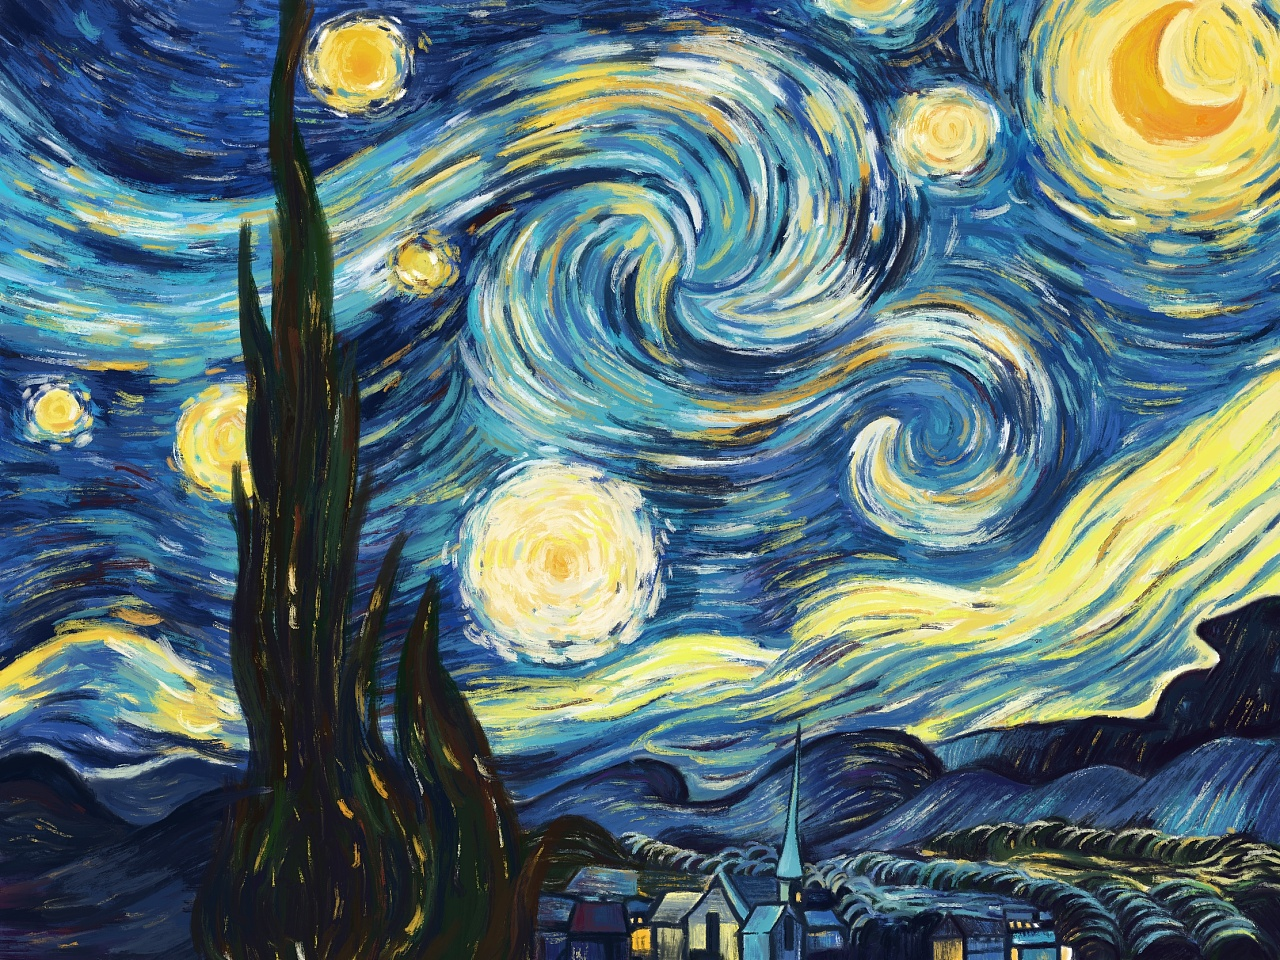
\includegraphics[width=0.8\textwidth]{figures/test}
	\caption{图片文字说明}
	\label{fig:test}
\end{figure}

\begin{lstlisting}[language=tex]
如图\ref{fig:test}所示。

\begin{figure}\label{fig:test}
	\centering
	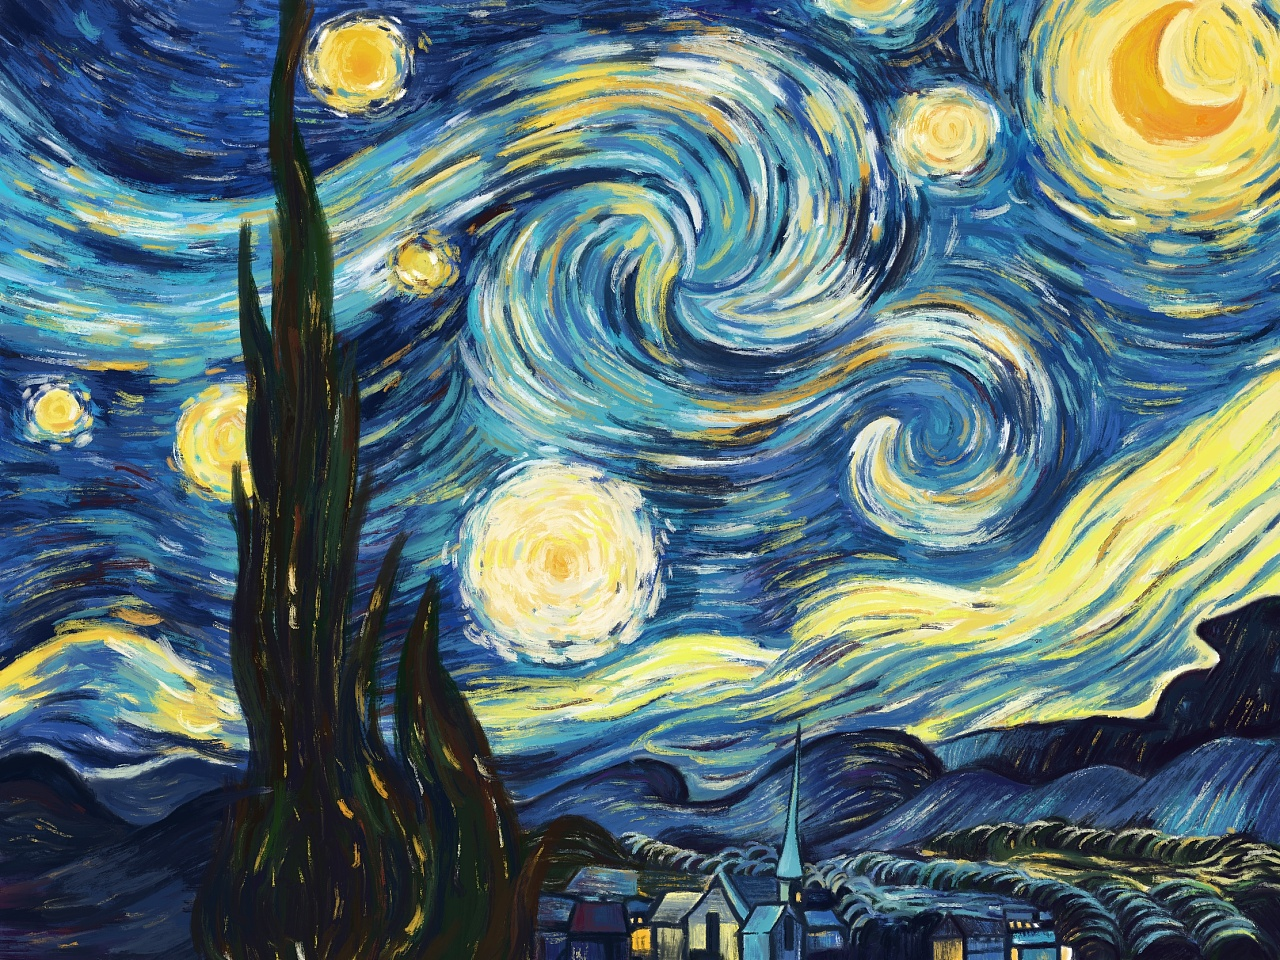
\includegraphics[width=0.8\textwidth]{figures/test}
\end{figure}
\end{lstlisting}

\section{公式}

如公式\ref{eq:test}所示。
\begin{equation}\label{eq:test}
	a^2+b^2=c^2
\end{equation}

\begin{lstlisting}[language=tex]
如公式\ref{eq:test}所示。% 注意这里没有空行
\begin{equation}\label{eq:test}
	a^2+b^2=c^2
\end{equation}
\end{lstlisting}

\section{代码}

行内代码:\lstinline|print|函数。

代码块:

\begin{lstlisting}[language=c]
int main() {
	printf("Hello World!\n");
	return 0;
}
\end{lstlisting}


\section{表格}

如表格\ref{tab:test}所示。

\begin{table}[H]\small
	\centering
	\caption{表头} \label{tab:test}
	\begin{tabular*}{0.3\textwidth}{@{\extracolsep{\fill}}cc}
		\toprule
		小写字母	&	大写字母	\\\midrule
		a		   &	A		\\
		b		   &	B   	\\	
		\bottomrule
	\end{tabular*}
\end{table}

\begin{lstlisting}[language=tex]
如表格\ref{tab:test}所示。

\begin{table}[H]\small
	\centering
	\caption{表头} \label{tab:test}
	\begin{tabular*}{0.5\textwidth}{@{\extracolsep{\fill}}cc}
		\toprule
		小写字母	&	大写字母	\\\midrule
		a		   &	A		\\
		b		   &	B   	\\	
		\bottomrule
	\end{tabular*}
\end{table}
\end{lstlisting}

\section{文献引用}

本文主要参考的文献有《一份(不太)简短的$\LaTeX$介绍》\cite{刘海洋2013LATEX},多个参考文献之间用英文逗号隔开。

\begin{lstlisting}[language=tex]
本文主要参考的文献有《一份(不太)简短的$\LaTeX$介绍》\cite{刘海洋2013LATEX},多个参考文献之间用英文逗号隔开。
\end{lstlisting}


